\chapter{System Design}

Current autonomous vehicles use the same architecture as the Urban DARPA Challenge vehicles did [1]?[4]. This architecture comprises three main processing modules, de- scribed below and illustrated in Fig. 1.

? The ?Perception+Localization? module combines data received from sensors and digital maps to estimate some relevant features representing the driving situation (e.g. position of other vehicles, road geometry).

? The ?Motion planner? selects the appropriate high-level behavior (e.g. car following, lane changing) and generates a trajectory corresponding to that behavior.

? The ?Trajectory controller? computes the steering and acceleration commands with the objective to follow the reference trajectory as closely as possible. These commands are sent to the actuators.

This architecture has been successfully used in the field of terrestrial robotics for decades.

Our autonomous driving framework combines two of the methods presented in the previous section: learning-by-demonstration, which is able to generate commands which feel natural to the passengers, and predictive control, which relies on model-based predictions to make decisions, and provides safety and stability. Our framework inherits the advantages of both. It is illustrated in Fig. 2, and the differences with the architecture in Fig. 1 are explained below.

? The trajectory generator is replaced by a driver model. The driver model uses learning-by-demonstration: it is trained using real driving data and can generate commands which imitate the driving style of the driver it learned from. In addition to the reference command, the motion planner out- puts a confidence value representing how reliable the reference command is. The confidence will be higher for driving situations which are similar to the training dataset.

? The trajectory controller is replaced by a model predictive controller which takes as an input the reference command generated by the driver model, and the associated confidence value. The role of the controller is to guarantee safety while trying to match the reference command sent by the driver model. When the confidence value is high and the safety constraints are respected, the command computed by the controller will match the reference command. The controller's command will deviate from the reference command when the confidence value is low or when a safety constraint violation is anticipated.

The driver model and the model predictive controller can be designed independently, and one can be modified at any time without impacting the performance of the other. This feature is particularly useful if one wants to adjust the car's driving style over time: the driver model can learn continuously, or be re- placed, without having to readjust any other module. One could also imagine extending the architecture in Fig. 2 to take advan- tage of cloud-based computing and learn new models based on data collected from millions of drivers.
The framework proposed above is general and can be applied to a variety of driving scenarios. Thus far, we have implemented and tested it for the longitudinal control of an autonomous car during lane keeping. In this scenario, the commanded input is the acceleration of the vehicle. The problem is defined formally below.

\begin{figure}[h]
\centering
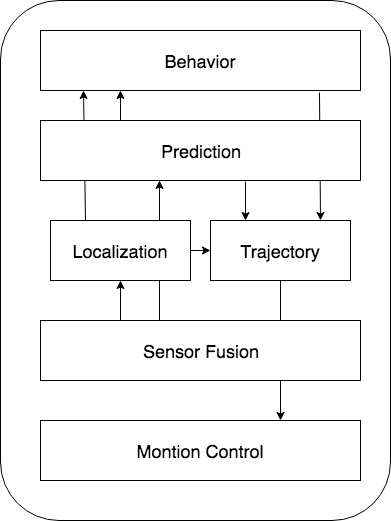
\includegraphics[width=0.5\textwidth]{figs/ch3/architecture}
\caption{Standard Architecture of Autonomous Vehicle Control.}
\end{figure}

\section{Behavior Planner}

\subsection{States for Autonomous Vehicles}


\section{Trajectory Generation}

The proposed path planning method is used to generate a safe and comfortable path (with an appropriate speed and acceleration) from an initial position towards a destination, while complying with a global route and map. Our method aims to resolve local path planning problems based on a global route and map. The global route is obtained by the high precision navigation system, and the map is downloaded from the Internet. As shown in Fig. 1, the map is composed of a set of way- points on the road edges and topology that describes the relationships between connected roads. The process by which the map is obtained falls outside the scope of this paper; therefore, the maps used in this paper are predefined in our simulations.

Fig. 1 shows the proposed dynamic path planning method, which includes three stages: center line construction, path candidate generation, and path selection. These are performed on the basis of perceived information and the proposed algorithms. As shown in Fig. 1, the center line of the road is constructed from the center waypoints, which are the center posi- tions of a pair of waypoints, using the method of cubic spline fitting. The path candidates, which are also described by the cubic spline, are generated by adjusting the lateral offset to the center line using the information for the current vehicle posi- tion, speed, and direction in the s   q coordinate system. During path selection, the costs of static safety, comfortability, and dynamic safety are taken into account, and are combined with information on road edges, and static and moving obstacles for selecting the optimal path. Our method provides not only the selected path, but also the appropriate speed and acceleration for the vehicle maneuvering system. In this study, the proposed dynamic path planning algorithm is executed 15 times per second, and a new path is generated from the current vehicle position at every time step.




A well known approach in tracking control theory is the Frenet Frame method, which asserts invariant tracking performance under the action of the special Euclidean group $SE(2) := SO(2) � R2$. Here, we will apply this method in order to be able to combine different lateral and longitudinal cost functionals for different tasks as well as to mimic human-like driving behavior on the highway. As depicted in Fig. 2, the moving reference frame is given by the tangential and normal vector ?tr , ?nr at a certain point of some curve referred to as the center line in the following. This center line represents either the ideal path along the free road, in the most simple case the road center, or the result of a path planning algorithm for unstructured environments [20]. Rather than formulating the trajectory generation problem directly in Cartesian Coordinates ?x, we switch to the pro- posed dynamic reference frame and seek to generate a one- dimensional trajectory for both the root point ?r along the center line and the perpendicular offset d with the relation

\subsection{Frenet Coordinates}

Frenet Coordinates are a way of representing position on a road in a more intuitive way than traditional (x,y) Cartesian Coordinates.
With Frenet coordinates, we use the variables s and d to describe a vehicle's position on the road. The s coordinate represents distance along the road (also known as longitudinal displacement) and the d coordinate represents side-to-side position on the road (also known as lateral displacement).
Why do we use Frenet coordinates? Imagine a curvy road like the one below with a Cartesian coordinate system laid on top of it...

\begin{figure}[h]
\centering
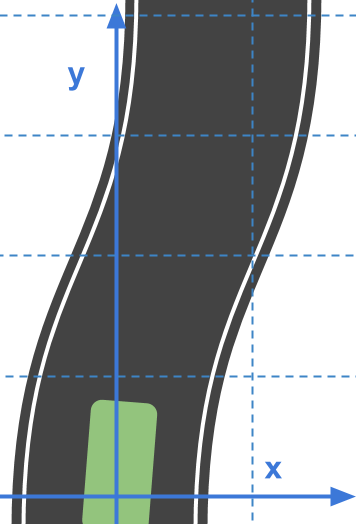
\includegraphics[width=0.5\textwidth]{figs/ch3/frenet-1}
\caption{Cropped input image.}
\end{figure}

Using these Cartesian coordinates, we can try to describe the path a vehicle would normally follow on the road...

\begin{figure}[h]
\centering
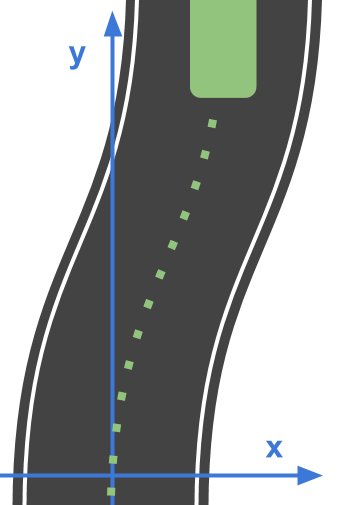
\includegraphics[width=0.5\textwidth]{figs/ch3/frenet-2}
\caption{Cropped input image.}
\end{figure}

\begin{figure}[h]
\centering
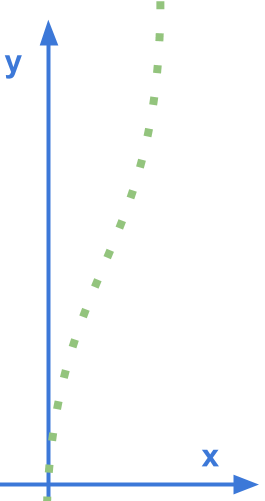
\includegraphics[width=0.5\textwidth]{figs/ch3/frenet-3}
\caption{Cropped input image.}
\end{figure}

And notice how curvy that path is! If we wanted equations to describe this motion it wouldn't be easy!
x(t)=?
y(t)=?
Ideally, it should be mathematically easy to describe such common driving behavior. But how do we do that? One way is to use a new coordinate system. Now instead of laying down a normal Cartesian grid, we do something like you see below...

\begin{figure}[h]
\centering
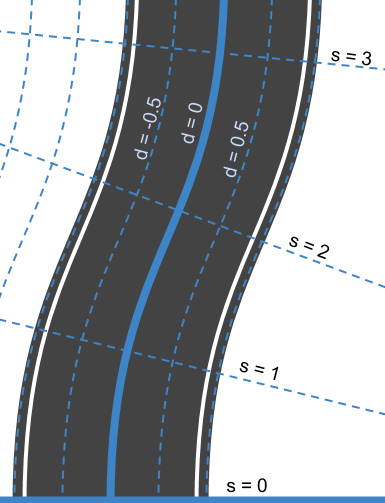
\includegraphics[width=0.5\textwidth]{figs/ch3/frenet-4}
\caption{Cropped input image.}
\end{figure}

Here, we've defined a new system of coordinates. At the bottom we have s=0 to represent the beginning of the segment of road we are thinking about and d=0 to represent the center line of that road. To the left of the center line we have negative d and to the right d is positive.
So what does a typical trajectory look like when presented in Frenet coordinates?

\begin{figure}[h]
\centering
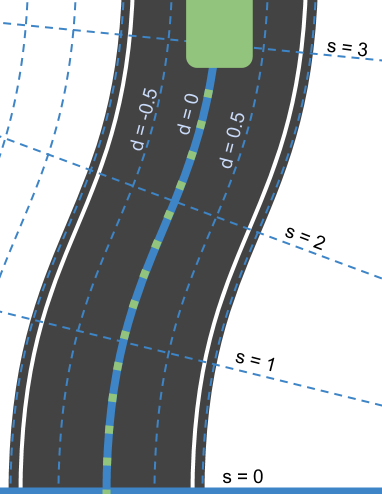
\includegraphics[width=0.5\textwidth]{figs/ch3/frenet-5}
\caption{Cropped input image.}
\end{figure}

\begin{figure}[h]
\centering
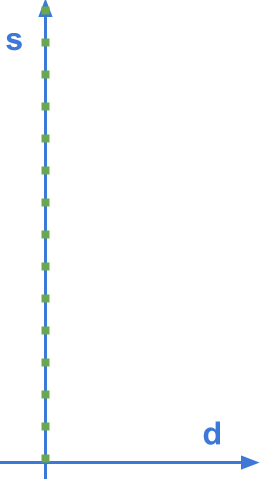
\includegraphics[width=0.5\textwidth]{figs/ch3/frenet-6}
\caption{Cropped input image.}
\end{figure}

It looks straight!
In fact, if this vehicle were moving at a constant speed of v0? we could write a mathematical description of the vehicle's position as:
s(t)=v0?t
d(t)=0

\begin{figure}[h]
\centering
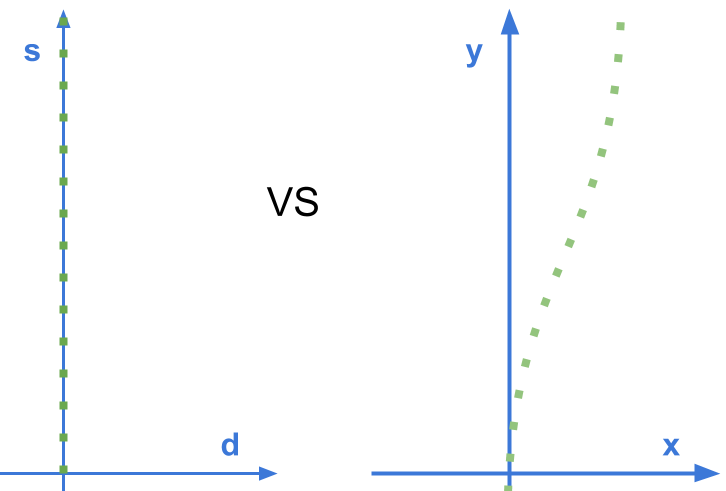
\includegraphics[width=0.5\textwidth]{figs/ch3/frenet-7}
\caption{Cropped input image.}
\end{figure}

...straight lines are so much easier than curved ones.


\subsection{Path candidates generation}

The path is the trajectory guiding the vehicle to follow a global route and avoid obstacles. The arc length s indicates the traveling distance on the global route, and the offset q can be used to measure the distance between the vehicle and an obstacle. Consequently, the proposed path planning method for avoiding obstacles is designed in the s   q coordinate system rather than the Cartesian coordinate system.

To use the direction and curvature of the center line, it is necessary to find the position of the vehicle on the center line, as shown in Fig. 2(b). We first map the vehicle position from the Cartesian coordinate system to the s   q coordinate system, and then determine the closest point of the center line p0, which has the minimum distance q. In this paper, a method combining quadratic minimization and Newton?s method is used to find p0 [41].

\subsection{Path candidates generation in the s   q coordinate system}
To generate path candidates, the curvature of each path is determined by the lateral offset q of the path, based on the
curvature of the center line. As shown in Fig. 3(a), Pinit is the original point on the center line. Pstart and Pend are the start and end points on the center line, respectively, for one step of planning. Pveh is the start point of the vehicle. P1 to P5 are the end points of five path candidates, and are indicated by r1 to r5. It is obvious that only r2;r4, and r5 are available and free of obstacles. The reason for this availability lies with the differences between the offset from the path candidate to the center line and the offset from the obstacle to the center line. Meanwhile, the positions of the obstacle and the vehicle on the center line can be expressed by the arc length s. In this case, it is necessary to design the algorithm to avoid obstacles using the parameters s and q. As shown in (4), a function describing the relationship between the arc length s and offset q is designed to provide a continuous change in the offset.

\subsection{Coordinates conversion of path candidate points}

Path candidates are generated in the s   q coordinate system, but path planning results must be mapped into a Cartesian coordinate system to convey to the maneuvering system. Path candidate points in the Cartesian coordinate system can be represented with respect to the arc length of the center line as (6) [43].

\section{Montrol Control}

\subsection{Waypoint Follower Node}
The waypoint follower node uses the $/final_waypoints$ data to publish $/twist_cmd$ for the dbw node to use. The node implementation uses an open source implementation of pure pursuit algorithm from Autoware. (https://github.com/CPFL/Autoware)

\subsection{Drive By Wire (DBW) Node}

An autonomous car require that actuators that control the motion of the vehicle, can be interacted with electronically. Therefore a drive-by-wire system is needed. A drive-by-wire system replaces the mechanical systems in a traditional vehicle by using electrical/electronic (E/E) systems to perform fundamental vehicle functions.

The drive-by-wire system includes steer-by-wire, brake-by-wire and throttle-by-wire. The "by- wire" expression means that the information, from the sensor to the actuator of the different systems, is transferred electronically through wires and not by traditional hydraulic systems or mechanically through struts or shafts.

The advantage of using drive-by-wire rather than mechanical systems is that reduction of cost, moving parts and weight can be achieved. Since the steering rack can be removed, the car?s shock impact, in case of a collision, can be improved. Using an electrical based system will also increase the information flow and ease up the interconnect between different components in the car, facilitating the use of safety functions such as; ABS (anti-lock brake system), ESP (electronic stability programme), etc.


The purpose of the drive by wire node is to publish commands to the vehicle actuators: steering wheel, accelerator, and break. The node subscribes to the following nodes:

${/current_velocity}$

$/twist_cmd$

$/vehicle/dbw_enabled$

It uses information from $current_velocity$ and $twist_cmd$ to determine the values to be sent to the actuators, while $/vehicle/dbw_enabled$ topic is only used to determine if drive-by-wire is being overridden, in which point it will stop publishing any message, and ignore the received messages.

The node delegates the actuator's value to the $twist_controller$ class, which returns a value for each of the actuators.

\subsubsection{Twist Controller}
The twist controller is initialized with values based on the vehicle configuration, as steer ratio and vehicle mass, and implements a single method control, which receives the vehicle target position and current velocity, and will return a value for acceleration, braking, and steering. It will in turn, delegate the calculation for each of those values to the $throttle_controller$, $brake_controller$, and $yaw_controller$. The $yaw_controller$ calculates a steering angle for every update, while the twist controller will calculate the position error (current - target) to determine if braking or acceleration should be engaged. If the error is positive, the throttle controller is used, while a negative error will be sent to the brake PID.

1) Throttle Controller ($throttle_controller.py$)
The throttle is initialized with a min and max acceleration values. It uses a PID controller to determine the amount of acceleration or decelaration to be given based on the difference between the target velocity and the current velocity.

2) Braking Controller ($braking_controller.py$)
The brake controller calculates the amount of torque to be sent to the brake by multiplying the vehicle mass, wheel radius and aceleration.

3) Steering Controller ($yaw_controller.py$)
The steering controller calculates the amount of steering it should send to the actuator using the target linear and angular velocity, taking into account the steer ratio of the vehicle.





%\bibliographystyle{plainnat}
%\markright{\textit{Bibliography}}
%\renewcommand{\chaptername}{}
%\bibliography{KL-Thesis}

%\end{flushleft}
%\vfill
